\documentclass[12pt]{article}
\usepackage[a4paper, margin=2cm]{geometry}
\usepackage[english]{babel} % To obtain English text with the blindtext package
\usepackage{blindtext}
\usepackage{graphicx} % Required for inserting images
\usepackage{array, multirow} % For extra column formatting
\usepackage{amsmath, amssymb, cancel} %for equation environment
\usepackage{float}
\usepackage{parskip} % For gaps between para
\usepackage{setspace}
\usepackage{pdfpages}
\usepackage{abstract}
\usepackage[export]{adjustbox}
\usepackage{emptypage}
\usepackage{tocloft}
\usepackage[nottoc]{tocbibind}
\usepackage{hyperref, url}
\usepackage[table]{xcolor}
\usepackage{minted}
    \usemintedstyle{monokai}
\usepackage{caption,subcaption}
    \captionsetup{font=footnotesize,labelfont=bf}
    \subcaptionsetup{font=footnotesize}
\usepackage{tcolorbox}
    \newtcolorbox{mintedbox}{
        colback=backcolour,
        boxrule=0pt,
        sharp corners,
        width=\linewidth,
        left=0pt, right=0pt,
        top=3pt, bottom=3pt
    }
\usepackage{cite}

\cftsetindents{section}{0em}{2em}
\cftsetindents{subsection}{0em}{2em}

\renewcommand\cfttoctitlefont{\hfill\Large\bfseries}
\renewcommand\cftaftertoctitle{\hfill\mbox{}}

\graphicspath{ {./images/} }

\definecolor{blurple}{HTML}{5865F2}
\definecolor{backcolour}{HTML}{272823}

\hypersetup{
    colorlinks=true,
    linkcolor=black,
    urlcolor=black,
    citecolor=blurple,
}

\urlstyle{same}

\pagenumbering{arabic}

\renewcommand{\arraystretch}{1.3}

\setcounter{secnumdepth}{5}
\setcounter{tocdepth}{5}
\newcommand\simpleparagraph[1]{%
  \stepcounter{paragraph}\paragraph*{\theparagraph\quad{}#1}}

%%%%%%%%%%%%%%%%%%%%%%%%%%%%%%%%%%%


\title{PHYC30170 Diffraction Pattern due to a Rectangular Aperture}
\author{Joana Adao}
\date{\today}

\begin{document}

\begin{titlepage}
    \begin{center}

        \begin{figure}[ht]
            
\includegraphics[width=\textwidth]{UCDLogo.png}
        \end{figure}
        
        \begin{figure}
            \centerline{
\includegraphics[width=\paperwidth]{UCDBanner.png}}
        \end{figure}

        \vspace{4cm}

        {\LARGE \bfseries PHYC30170 Physics Astro and Space Lab 1}\\
        \vspace{0.75cm}
        {\Large Diffraction Pattern due to a Rectangular Aperture}\\
        
        \vspace{1cm}
    
    {\Large \textbf{20 September 2025}}

    \vspace{2cm}
    
    {\large \textbf{by Joana C.C. Adao (Student No. 23311051)}}\\

    \end{center}
    
   \clearpage

\end{titlepage}


\tableofcontents
\thispagestyle{empty}

\newpage

\section*{Abstract}
\addtocontents{toc}{\protect\contentsline{section}{\textbf{Abstract}}{\hfill}{}}
\thispagestyle{empty}


\newpage

%%%%%%%%%%%%%%%%%%%%%%%%%%%%%%%%%%%

\setcounter{page}{1}
\section{Introduction} \label{sec:1}


\section{Theory} \label{sec:2}

\subsection{The Wave Nature of Light}

Light, an electromagnetic wave, is a transverse wave in such that it displaces the medium perpendicular to the direction of propagation.
Although the wave moves through the medium, the medium itself is not displaced by the wave and the atoms themselves remain near their equilibrium positions.
This is one of the key features that distinguishes waves from a stream of particles.
\cite{hecht2012optics}

\subsubsection{Spherical Waves}

An idealised point source of light emits radiation radially outwards and evenly in all directions, forming a spherical wavefront as shown in Figure (\ref{fig:1}).
The source is then described as isotropic, producing wavefronts that expand as concentric spheres increasing in diameter with distance from the source.
\cite{hecht2012optics}

For a spherically symmetrical description of this wavefront the descriptive function must depend only on the radial component \( r \) such that \cite{hecht2012optics,Born_Wolf_Bhatia_Clemmow_Gabor_Stokes_Taylor_Wayman_Wilcock_1999}:

\begin{equation} \label{eq:1}
    \psi(\vec{\mathbf{r}}) \; = \; \psi(r,\theta,\phi) \; =\; \psi(r)
\end{equation}

and for a harmonic spherical wave progressing radially outwards from the origin, the wave function is given by \cite{hecht2012optics}:

\begin{equation}\label{eq:2}
    \psi(r,t) = A \frac{\cos(kr - v t)}{r}
\end{equation}

with a constant speed \( v \) and \( A \) as the source strength, converging toward the origin. At any given value for time, this function corresponds to a set of concentric spheres extending through all space. \cite{hecht2012optics}

The electric field equation  at position \( r \) for a spherical wave of monochromatic light originating from a point source at position \( r_1 \) is given by \cite{reportguide7}:

\begin{equation} \label{eq:3}
    E(r,t) = \sum_{i=1}^N A \frac{\cos(k \lvert r-r_1 \rvert - \omega t)}{\lvert r - r_1 \rvert}
\end{equation}

where \( \lvert r - r_1 \rvert \) is the distance from the point source to the observation point, \( k = \frac{2\pi}{\lambda} \) is the wave number, \( \lambda \) is the wavelength of light, \( \omega = 2\pi f \) is the angular frequency and \( f \) is the frequency of light, with N wavelets superimposed. \cite{reportguide7}

This function for the wave can also be described in its complex form \cite{hecht2012optics}:

\begin{equation}\label{eq:4}
    E(r,t) = \left( \frac{A}{\lvert r-r_1 \rvert} \right) e^{i(k\lvert r -r_1 \rvert \;\pm\; \omega t)}
\end{equation}

The intensity observed corresponds to the time-averaged square of the electric field such that \cite{reportguide7}:

\begin{equation} \label{eq:5}
    I \propto \lvert E \rvert^2 \qquad \implies \qquad \overline{E^2} = \; \frac{1}{T} \int_0^T E^2 dt
\end{equation}

Equation (\ref{eq:2}) gives the general spherical wave solution, Equation (\ref{eq:3}) applying the same form to an electric field of light. Both show a dependency of amplitude \( A \) on \( \frac{1}{r} \), a diminishing amplitude with increasing distance.

\begin{figure}[H]
    \centering
    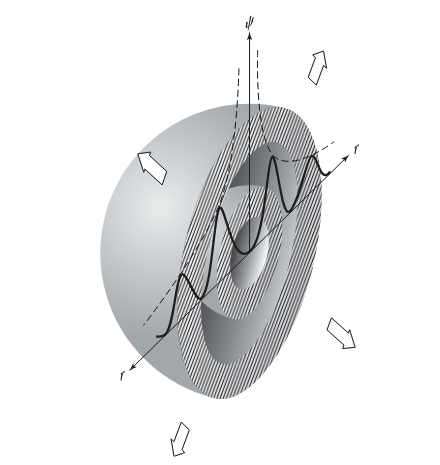
\includegraphics[width=.5\textwidth]{SphericalWavefront.png}
    \caption{Visual representation of a spherical wavefront from a point source; graph illustrates the amplitude decreasing with distance as the wave propagates radially outward. \cite{hecht2012optics}}
    \label{fig:1}
\end{figure}

\subsection{Huygens-Fresnel Principle} \label{sec:2.2}

Huygens Principle, or "Huygens-Fresnel Principle" states that each unobstructed point on a wavefront can be though of as an individual source of secondary spherical wavelets, each oscillating at the same frequency as the original wave,
as seen in Figure (\ref{fig:2}). \cite{hecht2012optics,enwiki:1291861847,likharev2013essential,Born_Wolf_Bhatia_Clemmow_Gabor_Stokes_Taylor_Wayman_Wilcock_1999}

The resulting optical field at any later point is then obtained by summing all the wavelets and taking into account their relative phases and amplitudes, building upon the superposition principle idea. \cite{hecht2012optics,Born_Wolf_Bhatia_Clemmow_Gabor_Stokes_Taylor_Wayman_Wilcock_1999}

\begin{figure}[H]
    \centering
    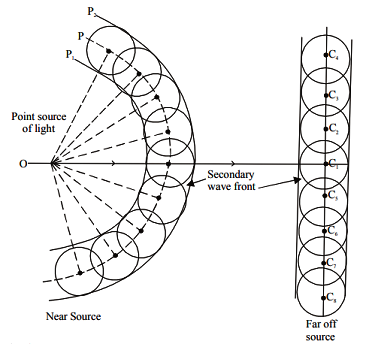
\includegraphics[width=.5\textwidth]{huygens.png}
    \caption{Diagram of Huygens' Principle for a near source (left) and far off source (right), showcasing the secondary wavelets at the secondary wavefront. \cite{huygensimgsource}}
    \label{fig:2}
\end{figure}

Applying this idea qualitatively it can be understood that for large wavelengths relative to an aperture, the waves spread widely into the region past the obstruction through diffraction.
Therefore, as the aperture size decreases, the diffracted waves take on an increasingly circular form and only then will the wavelets interfere constructively. \cite{hecht2012optics,Born_Wolf_Bhatia_Clemmow_Gabor_Stokes_Taylor_Wayman_Wilcock_1999}

\subsection{Diffraction}

Diffraction is the phenomenon of a wave, such as light, sound, or matter, bends or spreads out as it encounters an obstacle. When part of a wavefront is blocked or altered in amplitude or phase,
the waves that pass beyond that obstacle overlap and interfere with each other creating what is known as a \textbf{diffraction pattern}. \cite{hecht2012optics,Born_Wolf_Bhatia_Clemmow_Gabor_Stokes_Taylor_Wayman_Wilcock_1999}

\subsubsection{Fraunhofer vs. Fresnel Diffraction}

Expanding on the concept of diffraction, when a light is shined through a single small aperture in a screen, the light will make an image of the hole on another screen placed closely behind the first one with very faint surrounding fringes.
As the distance between the distance between both screens increases, the fringes become more visible, increasing in strength and detail, while the image of the hole is still prominent. This effect is known as \textbf{Fresnel} or \textbf{near-field} diffraction. \cite{hecht2012optics,enwiki:1291861847,cowley1995diffraction}

If the second screen continues to be moved farther away, the fringe pattern observed will change gradually. At a very large distance, the pattern spreads out so much that it bears very little resemblance
to the original aperture. This effect is known as \textbf{Fraunhofer} or \textbf{far-field} diffraction. \cite{hecht2012optics,cowley1995diffraction}

\begin{figure}[H]
    \centering
    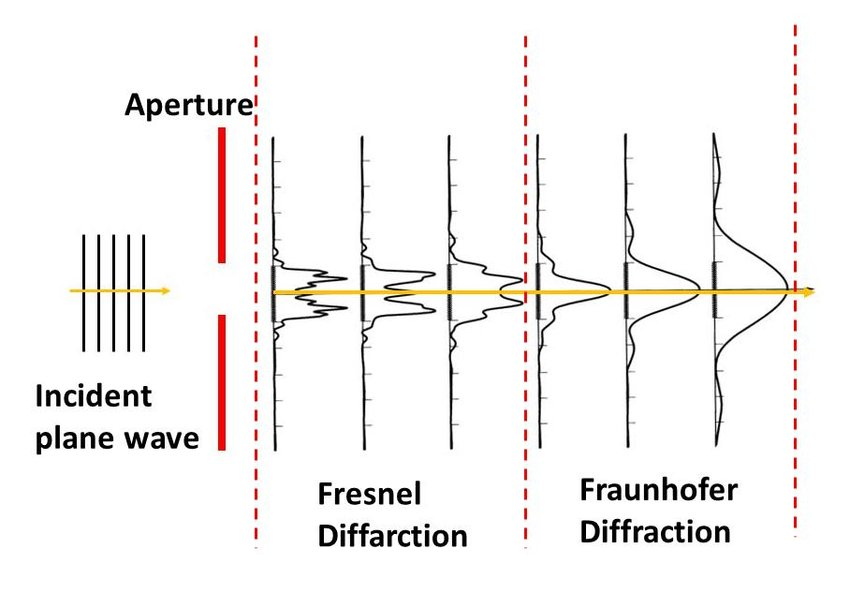
\includegraphics[width=.6\textwidth]{fraunfres.jpg}
    \caption{Intensity profiles in the near-field diffraction (middle) compared with the far-field diffraction (right) intensity profiles. \cite{phdthesis}}
    \label{fig:3}
\end{figure}

Both Fresnel and Fraunhofer diffraction can be understood as direct consequences of the Huygens-Fresnel Principle (§\ref{sec:2.2}). In the near-field, the curvature of the spherical wavelets is considered, giving rise
to the well-defined visible fringe patterns, while in the far-field the wavelets can be approximated to plane waves, leading to simpler and less defined diffraction patterns, see Figure (\ref{fig:3}). \cite{hecht2012optics}

\subsubsection{Diffraction for a Single Slit}

When coherent monochromatic light passes through a narrow slit it spreads out to form fringes on a screen. The pattern consists of a bright central maximum that's significantly wider and more intense
than the peripheral fringes. A series of alternating dark fringes (minima) and bright fringes (maxima) appear to either side. The peripheral maxima are only a small fraction of the intensity of the central maximum
that decreases rapidly with increasing distance to the centre, see Figure (\ref{fig:4}). \cite{hecht2012optics,Born_Wolf_Bhatia_Clemmow_Gabor_Stokes_Taylor_Wayman_Wilcock_1999,openstax3}

\begin{figure}[H]
    \centering
    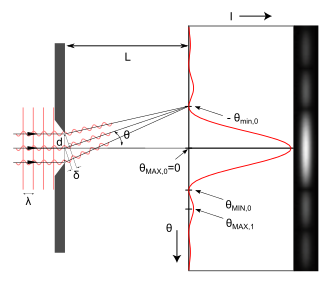
\includegraphics[width=.5\textwidth]{Single_Slit_Diffraction.png}
    \caption{Single slit diffraction diagram; infinitely many points (three) shown along length \textit{d} project phase contributions from the wavefront, producing a continuously varying intensity \( \theta \) on the registering plate. \cite{enwiki:1313573322}}
    \label{fig:4}
\end{figure}

\subsubsection{Diffraction for Two Slits}

When coherent monochromatic light passes through two closely spaced narrow slits the singular circular wavefront is split into two, each slit acting as a secondary source for the wavefronts that spread out and overlap.
The new secondary wavefronts maintain coherency and a constant phase relationship as they are derived from the same initial wave. The superposition of these wavefronts produces a pattern of alternating dark and bright fringes
when projected onto a screen. The central maximum remains the brightest and most intense, with the fringes decreasing in intensity with increasing distance from the centre (as with the single slit), see Figure (\ref{fig:5}). This diffraction pattern was first demonstrated in
Thomas Young's 1801 experiment. \cite{hecht2012optics,openstax3,10.11648/j.ajop.20190701.11}

\begin{figure}[H]
    \centering
    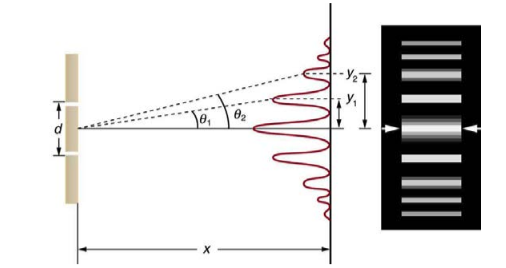
\includegraphics[width=.65\textwidth]{youngs slit.png}
    \caption{Double slit diffraction diagram; intensity falls off with angle to form an interference pattern consisting of a series of bright and dark fringes. \cite{openstax3}}
    \label{fig:5}
\end{figure}

\subsubsection{Diffraction for a Circular Aperture}

When coherent monochromatic light passes through a small circular aperture the pattern that appears is of a bright central spot maxima surrounded by fuzzy, airy concentric rings
decreasing in intensity with increasing distance from the centre. The central disc is the most intense and the intensity of the surrounding rings is dependant on the size of the aperture.
Rings become more regular and defined in the far-field (Fraunhofer) regime, notably more complex and less defined when in the near-field (Fresnel) regime, see Figure (\ref{fig:6}). Deviations from the usual pattern arise 
if coherence is not perfect, if the aperture size is comparable to the wavelength, or if the illumination is non-uniform. \cite{openstax3,andrews1947diffraction,burch1985fresnel,koushki2019diffraction}

\begin{figure}[H]
    \centering
    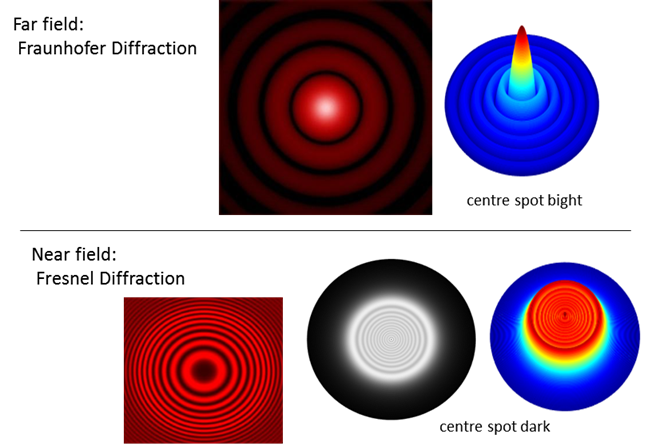
\includegraphics[width=.65\textwidth]{circularapert.png}
    \caption{Circular aperture diffraction pattern; Fraunhofer (far-field) diffraction (top), Fresnel (near-field) diffraction (bottom) where a central black spot can be observed. \cite{VisualPhysics_singleSlit}}
    \label{fig:6}
\end{figure}

\section{Experimental Setup \& Procedure} \label{sec:3}


\section{Results} \label{sec:4}



\section{Analysis \& Discussion} \label{sec:5}



\section{Conclusion} \label{sec:6}


\newpage

%%%%%%%%%%%%%%%%%%%%%%%%%%%%%%%%%%%

\section*{Appendix} \label{sec:A}
\addcontentsline{toc}{section}{Appendix}

\bibliographystyle{IEEEtran}
\bibliography{PHYC30170References} \label{sec:ref}

\vspace{1.5cm}


\end{document}